\documentclass[tikz,border=3.14mm]{standalone}
\begin{document}
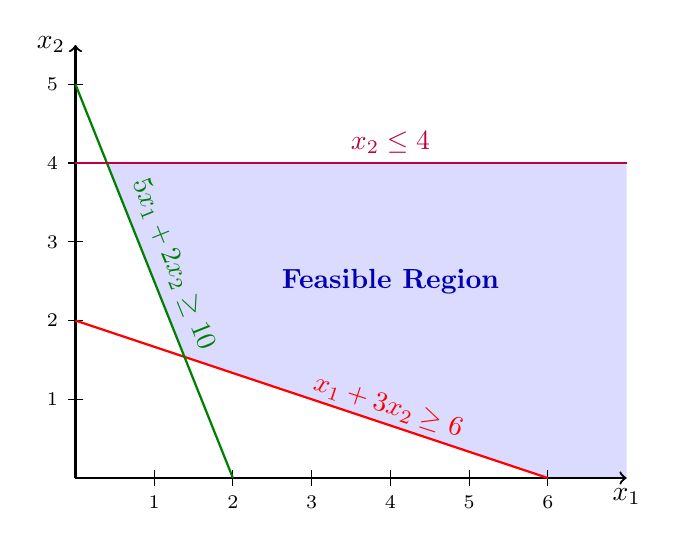
\begin{tikzpicture}

    % Highlight the feasible region
    \fill[blue!20,opacity=0.7] 
        (0.4,4) -- (1.39,1.55)  -- (6,0) -- (7,0) -- (7,4) -- cycle;

    % Define axes
    \draw[thick,->] (0,0) -- (7,0) node[anchor=north] {$x_1$};
    \draw[thick,->] (0,0) -- (0,5.5) node[anchor=east] {$x_2$};

    % Add tick marks on the x_1-axis
    \foreach \x in {1,2,3,4,5,6} {
        \draw (\x,0.1) -- (\x,-0.1) node[anchor=north] {\scriptsize $\x$};
    }

    % Add tick marks on the x_2-axis
    \foreach \y in {1,2,3,4,5} {
        \draw (0.1,\y) -- (-0.1,\y) node[anchor=east] {\scriptsize $\y$};
    }

    % Define the constraints
    % Line 1: X + 3Y = 6
    \draw[red,thick] (0,2) -- (6,0);
    \node[red, rotate=-18, anchor=north west] at (3,1.5) {$x_1 + 3x_2 \geq 6$};

    % Line 2: 5X + 2Y = 10
    \draw[green!50!black,thick] (0,5) -- (2,0);
    \node[green!50!black, rotate=-68, anchor=north west] at (1,4) {$5x_1 + 2x_2 \geq 10$};

    % Line 3: Y = 4
    \draw[purple,thick] (0,4) -- (7,4);
    \node[purple, rotate=0, anchor=south] at (4,4) {$x_2 \leq 4$};

    % Label feasible region
    \node[blue!70!black, font=\bfseries] at (4,2.5) {Feasible Region};

    % Mark intersection points
%    \fill[black] (0,4) circle (2pt) node[anchor=east] {\scriptsize $(0,4)$};
%    \fill[black] (6,0) circle (2pt) node[anchor=north] {\scriptsize $(6,0)$};

\end{tikzpicture}
\end{document}
